\documentclass[12,french]{report}
\usepackage{geometry}
\geometry{vmargin=3cm, hmargin=3cm}
\usepackage[T1]{fontenc}
\usepackage[utf8]{inputenc}
\usepackage[french]{babel}
\usepackage{graphicx}
\usepackage{amsmath}
\usepackage{amssymb}
\usepackage{sectsty}
\usepackage{authblk}
\usepackage{algpseudocode}
\usepackage{algorithm}
\usepackage{xspace}
\usepackage{mathtools}
\usepackage{mathrsfs}
\usepackage{enumitem}
\usepackage{titlesec}
\usepackage{hyperref}
\usepackage{xcolor}
\usepackage[justification=centering]{caption}
\usepackage{float}
\usepackage{tabto}

\usepackage{listings}
\usepackage{cleveref}

\renewcommand{\lstlistingname}{Code}
%\renewcommand{\figurename}{Fig.}

\lstdefinestyle{chstyle}{%
backgroundcolor=\color{gray!12},
basicstyle=\ttfamily\small,
showstringspaces=false,
numbers=left}

%\AddThinSpaceBeforeFootnotes
%\FrenchFootnotes

\titleformat{\chapter}[hang]{\bf\Huge}{\thechapter.}{2pc}{}
\titlespacing*{\chapter}{10pt}{0pt}{40pt}[0pt]
\newcommand{\HRule}{\rule{\linewidth}{0.5mm}}

\providecommand{\keywords}[1]{\textbf{\textit{Keywords:}} #1}
\bibliographystyle{apalike}

\usepackage{hyperref}

\begin{document}
\hypersetup{pdfborder=0 0 0}

\begin{titlepage}

\begin{center}
	\vspace*{\stretch{1}}
	\textsc{{\LARGE Institut national des sciences appliquées de Rouen} \\ 			\vspace{6mm} {\Large INSA de Rouen}} \\
	\vspace{5mm}
	
\includegraphics[width=0.4\textwidth]{./Images/insa}\\[1.0 cm]

	\textsc{\Large Mini-projet COO - GM3}\\[0.6cm]

	% Title
	\HRule \\[0.5cm]
	{ \Huge \bfseries Réalisation d'un jeu de dames en Java}\\[0.2cm]
	\HRule \\[0.75cm]

	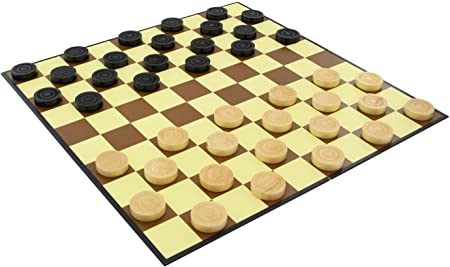
\includegraphics[width=0.7\textwidth]{./Images/Page_de_garde}\\[0.9 cm]

	% Author and supervisor
	\begin{minipage}{0.4\textwidth}
		\begin{flushleft} \large
			\emph{Auteurs:}\\
			Thibaut \textsc{André-Gallis} \\
			{\small\href{mailto:thibaut.andregallis@insa-rouen.fr}{thibaut.andregallis@insa-rouen.fr}} \\
			Kévin \textsc{Gatel} \\
			{\small\href{mailto:kevin.gatel@insa-rouen.fr}{kevin.gatel@insa-				rouen.fr}}
		\end{flushleft}
	\end{minipage}
	\begin{minipage}{0.4\textwidth}
		\begin{flushright} \large
			\emph{Enseignants:} \\
			Mathieu \textsc{Bourgais} \\
			{\small\href{mailto:mathieu.bourgais@insa-rouen.fr}								{mathieu.bourgais@insa-rouen.fr}}\\
			Habib \textsc{Abdulrab} \\
			{\small\href{mailto:habib.abdulrab@insa-rouen.fr}{habib.abdulrab@insa-rouen.fr}}
		\end{flushright}
	\end{minipage}
	\vspace*{\stretch{1}}

	\vfill
	{\large 16 Mai 2021}
\end{center}
\end{titlepage}

\tableofcontents

%\listoffigures

\renewcommand{\chaptername}{}
\chapter*{Introduction}

Le mini-projet que nous avons choisi est la réalisation du jeu de dames en Java.\\

Le jeu de dames est un célèbre jeu de réflexion joué à deux inventé pour la première fois en Egypte antique vers -1500 avant J-C.
Pour la version classique, le jeu de dames est composé d'un damier de 10 cases sur 10 cases de deux couleurs alternées et d'une vingtaine de pions par joueur disposés les uns en face des autres. Il existe également des variantes de ce jeu qui utilisent des damiers de 64 cases (8 sur 8) et 144 cases (12 par 12). 
Le but du jeu est alors de capturer ou d'immobiliser toutes les pièces du joueur adverse. \\

Le but de ce projet est d'utiliser habilement les concepts de la programmation objet, c'est-à-dire savoir écrire les différents diagrammes, maîtriser l'héritage entre les classes, le polymorphisme, la gestion des interfaces ou des classes arbitraires, etc...\\

Pour bien répondre au problème, nous allons d'abord regarder le \textbf{diagramme UML} et le \textbf{diagramme de cas} (Use-cases) afin de comprendre l'organisation du code.\\

Ensuite, nous allons présenter et décrire le rôle de \textbf{chacune des classes} qui ont été nécessaires à la réalisation du projet.\\

Enfin, nous verrons \textbf{les différents problèmes} que nous avons pu rencontrer lors de la programmation du jeu.


\chapter{Les diagrammes}

\section{UML}

\section{Use-cases}

\chapter{Les classes}

\chapter{Problèmes rencontrés}

\chapter*{Conclusion}
\addcontentsline{toc}{chapter}{Conclusion}

\chapter*{Annexe}

\end{document}
